%%%%%%%%%%%%%%%%%%%%%%%%%%%%%%%%%%%%%%%%%%%%%%%%%%%%%%%%%%%%%%%%%%%%%%%%%%%%%%%%%%%%%%%%%%%%%%%%%%%%%%%%%%%%%%%%%%%%%%%%%%%%%%
%%% Template para de LaTeX para o evento 12º Congresso Iberoamericano de Acústica (12º Congreso Iberoamericano de Acústica)
%%%                      em conjunto com XXIX Encontro da SOBRAC (XXIX Encontro de la SOBRAC)
%%% Baseado no modelo da Revista Acústica e Vibrações da SOBRAC
%%% Release 25/03/2021
%%%	Desenvolvido por por Prof. William D'Andrea Fonseca, Dr. Eng. - Engenharia Acústica UFSM
%%% will.fonseca@eac.ufsm.br
%%%%%%%%%%%%%%%%%%%%%%%%%%%%%%%%%%%%%%%%%%%%%%%%%%%%%%%%%%%%%%%%%%%%%%%%%%%%%%%%%%%%%%%%%%%%%%%%%%%%%%%%%%%%%%%%%%%%%%%%%%%%%%
\documentclass[12pt, a4paper, twoside, twocolumn]{article}
%%%%%%%%%%%%%%%%%%%%%%%%%%%%%%%%%%%%%%%%%%%%%%%%%%%%%%%%%%
%%% Input
\usepackage[utf8]{inputenc} 
\usepackage[english,spanish,brazil]{babel} % Select the options that fit your needs.
\usepackage[T1]{fontenc}
\usepackage{lmodern, mathptmx} % For Times New Roman
%%%%%%%%%%%%%%%%%%%%%%%%%%%%%%%%%%%%%%%%%%%%%%%%%%%%%%%%%%%%%%%%%%%%%%%%%%%%%%%%%%%%%%%%%%%%%%%%%%%%%%%%%%%%%%%%%%%%
\usepackage{FIA2020} %%% Template basics
%%%%%%%%%%%%%%%%%%%%%%%%%%%%%%%%%%%%%%%%%%%%%%%%%%%%%%%%%%%%%%%%%%%%%%%%%%%%%%%%%%%%%%%%%%%%%%%%%%%%%%%%%%%%%%%%%%%%
%%% Select language options

% For spanish words uncomment the line below
%\Resumen

% For paper only in English uncomment the line below
% \SuppressResumo 
%%%%%%%%%%%%%%%%%%%%%%%%%%%%%%%%%%%%%%%%%%%%%%%%%%%%%%%%%%%%%%%%%%%%%%%%%%%%%%%%%%%%%%%%%%%%%%%%%%%%%%%%%%%%%%%%%%%%
%%% Paper data

\Authors{Fonseca,~W.~D'A.; Last~name,~I.} % For PDF metadata

% Use the structure Last name, I
\AuthorsAffiliations{Fonseca,~W.~D'A.$^1$; Sobrenome,~N.$^2$} % Use numbers to mark the affiliations

%% Use one line for each author of different affiliations. 
%% If authors share the same affiliation, use the same data and declare different emails.
\Affiliations{$^1$\,Engenharia Acústica, Universidade Federal de Santa Maria, Santa Maria, RS, Brasil, will.fonseca@eac.ufsm.br\\[2pt]  
$^2$\,Laboratório de Vibrações, Instituição, Cidade, Estado, País, nome@dominio.br}

\TittleComplete{Instruções e modelo de artigo para o FIA 2020 e\\ XXIX Encontro da Sobrac}
\TitleShort{Instruções e modelo de artigo para o FIA 2020 e XXIX Sobrac}              % Short title for the heaing
\TitleEnglish{Instructions and article template for FIA 2020 and XXIX Sobrac meeting} % Title in English for papers in Portuguese or Spanish

\PalavrasChave{artigo técnico, FIA, Sobrac, acústica, vibrações} % o Palavras claves
\Keywords{technical paper, FIA, Sobrac, acoustics, vibration}

\PACS{look the instructions inside this template}

\Resumo{Esse campo é destinado ao resumo do artigo que deve ter entre 180 e 300 palavras.
O resumo, palavras-chave, PACS, \textit{title}, \textit{abstract} e \textit{keywords} devem ser colocados na primeira página do artigo, buscando não se estender para outra página.  O resumo deve fazer uma apresentação concisa do artigo técnico científico, contendo, uma introdução, o objetivo, uma síntese da metodologia, o principal resultado e a principal conclusão (preferencialmente nessa ordem). Não é necessário separar em itens ou seções dentro do resumo. Assim, o leitor pode conhecer a essência do conteúdo do artigo. Lembre-se que o resumo é como o \textit{trailer} de um filme, as pessoas ficarão interessadas em ler completamente o artigo se o resumo lhes interessar. O resumo não deve conter informações novas não contidas no artigo; abreviações indefinidas; discussão prévia de outra literatura; referências e citações e excesso de detalhes acerca dos métodos empregados. Ele também não é o parágrafo de introdução do documento, isso deve ser colocado no início do texto. Utilize apenas informações úteis e relevantes, faça um exercício de empatia com o possível leitor interessado. Para se obter um resumo coeso, elegante e de acordo com o artigo, escreva uma prévia, realize a escrita completa do documento e, ao final, revise-o observando se o conteúdo dele reflete de forma consistente o teor do documento. Seguindo o resumo, o autor deve listar até cinco palavras chaves (evite colocar as mesmas palavras que formam o título do artigo). Após essa etapa, há ainda os PACS, que são um sistema de classificação hierárquica (mais detalhes no texto) e, em conseguinte, título, resumo e palavras-chave em inglês.}

\Abstract{
This field is intended for the abstract of the article that must contain between 180 and 300 words. The items \textit{resumo}, \textit{palavras-chave}, PACS, title, abstract, and keywords should constitute the first page (i.e. avoid extending them to the following page). The abstract should make a concise presentation of the scientific-technical article, containing an introduction, the objective, a synthesis of the methodology, the main result and the final conclusion (preferably in that order). No separate items or sections are required within the abstract. Thus, the reader may acknowledge the essence of the article content. Remember that the abstract is like a movie trailer, people will consider reading the complete article if the abstract is interesting. The abstract should not contain new information not contained within the article; undefined abbreviations; previous discussion of another literature; references and citations or excessive detail about the methods employed. It is also not the introductory paragraph of the work; this should be placed at the beginning of the text. Use only relevant and useful information, exercising empathy with prospective readers. For a cohesive, elegant abstract that represents the article, write a preview, write the paper completely, and then review it by looking at whether its content consistently reflects the content of the document. Following the abstract, the author should list up to five keywords (avoid using the same words contained in the article’s title). After this step, there are also the PACS, which are a hierarchical classification system (more details within the text) and, finally, title, abstract and keywords in English (PACS are only put after \textit{resumo} in Portuguese contributions).}

\Metadata % Includes the metada into the PDF
%%%%%%%%%%%%%%%%%%%%%%%%%%%%%%%%%%%%%%%%%%%%%%%%%%%%%%%%%%%%%%%%%%%%%%%%%%%%%%%%%%%%%%%%%%%%%%%%%%%%%%%%%%%%%%%%%%%%
%%%%%%%%%%%%%%%%%%%%%%%%%%%%%%%%%%%%%%%%%%%%%%%%%%%%%%%%%%%%%%%%%%%%%%%%%%%%%%%%%%%%%%%%%%%%%%%%%%%%%%%%%%%%%%%%%%%%
\begin{document} \setcounter{page}{1} %%%%%%%%%%%%%%%%%%%%%%%%%%%%%%%%%%%%%%%%%%%%%%%%%%%%%%%%%%%%%%%%%%%%%%%%%%%%%%%%%%%%%%%%%%%%%%%%%%%%%%%%%%%%%%%%%%%%
%%% Template para de LaTeX para o evento 12º Congresso Iberoamericano de Acústica 
%%%                      em conjunto com XXIX Encontro da Sobrac
%%% Baseado no modelo da Revista Acústica e Vibrações da Sobrac
%%% Release 19/04/2022
%%%	Desenvolvido por por Prof. William D'Andrea Fonseca, Dr. Eng. - Engenharia Acústica UFSM
%%% will.fonseca@eac.ufsm.br
%%%%%%%%%%%%%%%%%%%%%%%%%%%%%%%%%%%%%%%%%%%%%%%%%%%%%%%%%%%%%%%%%%%%%%%%%%%%%%%%%%%%%%%%%%%%%%%%%%%%%%%%%%%%%%%%%%%%
%%%%%%%%%%%%%%%%%%%%%%%%%%%%%%%%%%%%%%%%%%%%%%%%%%%%%%%%%%%%%%%%%%%%%%%%%%%%%%%%%%%%%%%%%%%%%%%%%%%%%%%%%%%%%%%%%%%%
%% Estilo do artigo
\pagestyle{plain}
%%%%%%%%%%%%%%%%%%%%%%%%%%%%%%%%%%%%%%%%%%%%%%%%%%%%%%%%%%%%%%%%%%%%%%%%%%%%%%%%%%%%%%%%%%%%%%%%%%%%%%%%%%%%%%%%%%%%
%%% Primeira página
\thispagestyle{firststyle}
% \newgeometry{top=2.1cm, bottom=2cm, left=1.9cm, right=1.9cm, headsep=5mm}
%%%%%%%%%%%%%%%%%%%%%%%%%%%%%%%%%%%%%%%%%%%%%%%%%%%%%%%%%%%%%%%%%%%%%%%%%%%%%%%%%%%%%%%%%%%%%%%%%%%%%%%%%%%%%%%%%%%%
\begin{textblock}{200}(150.2,283.51)
\fontsize{8}{8}\selectfont\sffamily 
DOI:~\href{https://doi.org/\DOIArtigo}{\DOIArtigo}
\end{textblock}
%%% Título
\begin{textblock}{170}(37,12)

\includegraphics[width=0.82\textwidth,page=1]{FIA-logo.pdf}
\end{textblock}

\twocolumn[
\begin{@twocolumnfalse}
\vspace{60pt}
\begin{center}
{\fontsize{18}{22}\selectfont\bfseries 
%% Título
%%%%%%%%%%%%%%%%%%%%%%%%%%%%%%%%%%%%%%%%%%%%%%%%%%%%%%%%%%%%%%%%%%%%%%%%%%%%%%%%%%%%%%%%%%%%%%%%%%%%%%%%%%%%%%%%%%%%
\TituloCompletoArtigo \bookmark[page=1,level=1]{Título e Resumo}
%%%%%%%%%%%%%%%%%%%%%%%%%%%%%%%%%%%%%%%%%%%%%%%%%%%%%%%%%%%%%%%%%%%%%%%%%%%%%%%%%%%%%%%%%%%%%%%%%%%%%%%%%%%%%%%%%%%%
\par}

%%%%%%%%%%%%%%%%%%%%%%%%%%%%%%%%%%%%%%%%%%%%%%%%%%%%%%%%%%%%%%%%%%%%%%%%%%%%%%%%%%%%%%%%%%%%%%%%%%%%%%%%%%%%%%%%%%%
%%%%%%%%%%%%%%%%%%%%%%%%%%%%%%%%%%%%%%%%%%%%%%%%%%%%%%%%%%%%%%%%%%%%%%%%%%%%%%%%%%%%%%%%%%%%%%%%%%%%%%%%%%%%%%%%%%%
\vspace{12pt}
{\fontsize{11}{13}\selectfont \bfseries 
%% Autores
%%%%%%%%%%%%%%%%%%%%%%%%%%%%%%%%%%%%%%%%%%%%%%%%%%%%%%%%%%%%%%%%%%%%%%%%%%%%%%%%%%%%%%%%%%%%%%%%%%%%%%%%%%%%%%%%%%%
\AutoresFiliacoesArtigo
%%%%%%%%%%%%%%%%%%%%%%%%%%%%%%%%%%%%%%%%%%%%%%%%%%%%%%%%%%%%%%%%%%%%%%%%%%%%%%%%%%%%%%%%%%%%%%%%%%%%%%%%%%%%%%%%%%%
\par}

\vspace{2mm}
{\fontsize{9}{11}\selectfont 
%% Filiações
%%%%%%%%%%%%%%%%%%%%%%%%%%%%%%%%%%%%%%%%%%%%%%%%%%%%%%%%%%%%%%%%%%%%%%%%%%%%%%%%%%%%%%%%%%%%%%%%%%%%%%%%%%%%%%%%%%%
\FiliacoesArtigo
%%%%%%%%%%%%%%%%%%%%%%%%%%%%%%%%%%%%%%%%%%%%%%%%%%%%%%%%%%%%%%%%%%%%%%%%%%%%%%%%%%%%%%%%%%%%%%%%%%%%%%%%%%%%%%%%%%%%
\par}
\end{center}

\vspace{-5mm}{\color{FIABlue}\rule{\textwidth}{0.4pt}}
%%%%%%%%%%%%%%%%%%%%%%%%%%%%%%%%%%%%%%%%%%%%%%%%%%%%%%%%%%%%%%%%%%%%%%%%%%%%%%%%%%%%%%%%%%%%%%%%%%%%%%%%%%%%%%%%%%%%
%%%%%%%%%%%%%%%%%%%%%%%%%%%%%%%%%%%%%%%%%%%%%%%%%%%%%%%%%%%%%%%%%%%%%%%%%%%%%%%%%%%%%%%%%%%%%%%%%%%%%%%%%%%%%%%%%%%%
%%% Resumo e palavras-chave
\ResumoTexto
%%%%%%%%%%%%%%%%%%%%%%%%%%%%%%%%%%%%%%%%%%%%%%%%%%%%%%%%%%%%%
%%% Title, abstract and keywords
%%%%%%%%%%%%%%%%%%%%%%%%%%%%%%%%%%%%%%%%%%%%%%%%%%%%%%%%%%%%%
%%% Title
\begin{otherlanguage*}{english}
{\EnglishTitle}
%%%%%%%%%%%%%%%%%%%%%%%%%%%%%%%%%%%%%%%%%%%%%%%%%%%%%%%%%%%%%%%%%%%%%%%%%%%%%%%%%%%%%%%%%%%%%%%%%%%%%%%%%%%%%%%%%%%%
%%%%%%%%%%%%%%%%%%%%%%%%%%%%%%%%%%%%%%%%%%%%%%%%%%%%%%%%%%%%%%%%%%%%%%%%%%%%%%%%%%%%%%%%%%%%%%%%%%%%%%%%%%%%%%%%%%%%
%%% Abstract
		{\textbf{Abstract}} \vspace{5pt}
		
		{\fontsize{11}{12.5}\selectfont
		\AbstractArtigo
		\par}
		%%%%%%%%%%%%%%%%%%%%%%%%% Keywords
		\vspace{0.7\baselineskip} \fontsize{11}{12}\selectfont
		\textbf{Keywords: }{\fontsize{11}{12}\selectfont 
		\KeywordsArtigo.
		\par}
		%%%%%%%%%%%%%%%%%%%%%%%%% PACs:
		\PACSEnglish
	  \vspace{6mm}
\end{otherlanguage*}		
%%%%%%%%%%%%%%%%%%%%%%%%%%%%%%%%%%%%%%%%%%%%%%%%%%%%%%%%%%%%%%%%%%%%%%%%%%%%%%%%%%%%%%%%%%%%%%%%%%%%%%%%%%%%%%%%%%%%
%%%%%%%%%%%%%%%%%%%%%%%%%%%%%%%%%%%%%%%%%%%%%%%%%%%%%%%%%%%%%%%%%%%%%%%%%%%%%%%%%%%%%%%%%%%%%%%%%%%%%%%%%%%%%%%%%%%%
\end{@twocolumnfalse}
]
% \restoregeometry 
% \newgeometry{top=2.1cm, bottom=2cm, left=1.9cm, right=1.9cm, headsep=5mm}
\pagestyle{plain}

%%%%%%%%%%%%%%%%%%%%%%%%%%%%%%%%%%%%%%%%%%%%%%%%%%%%%%%%%%%%%%%%%%%%%%%%%%%%%%%%%%%%%%%%%%%%%%%%%%%%%%%%%%%%%%%%%%%%
% EOF

%%%%%%%%%%%%%%%%%%%%%%%%%%%%%%%%%%%%%%%%%%%%%%%%%%%%%%%%%%%%%%%%%%%%%%%%%%%%%%%%%%%%%%%%%%%%%%%%%%%%%%%%%%%%%%%%%%%%
%%%%%%%%%%%%%%%%%%%%%%%%%%%%%%%%%%%%%%%%%%%%%%%%%%%%%%%%%%%%%%%%%%%%%%%%%%%%%%%%%%%%%%%%%%%%%%%%%%%%%%%%%%%%%%%%%%%%
%%% ARTIGO
%%%%%%%%%%%%%%%%%%%%%%%%%%%%%%%%%%%%%%%%%%%%%%%%%%%%%%%%%%%%%%%%%%%%%%%%%%%%%%%%%%%%%%%%%%%%%%%%%%%%%%%%%%%%%%%%%%%%
%%%%%%%%%%%%%%%%%%%%%%%%%%%%%%%%%%%%%%%%%%%%%%%%%%%%%%%%%%%%%%%%%%%%%%%%%%%%%%%%%%%%%%%%%%%%%%%%%%%%%%%%%%%%%%%%%%%%
\clearpage % Recomenda-se deixar apenas os dados de resumo da primeira página, porém, isso não é obrigatório.

\section{Introdução}

Este texto de instruções modelo foi elaborado para que os autores possam apresentar os artigos de forma padronizada. 
Ele foi adaptado do modelo da Revista Acústica e Vibrações (da Sobrac), sendo de uso para o 12º Congresso Iberoamericano de Acústica integrado com o  XXIX Encontro da Sobrac.
%
Isso proporcionará uma uniformidade da formatação para os artigos completos do evento.
Neste modelo são apresentadas as principais diretrizes para a elaboração do artigo completo no que diz respeito à apresentação de conteúdo, gráfica, estrutura, diagramação e ao procedimento para a submissão dos artigos. 
Este documento já conta com a formatação de estilos personalizados para a elaboração do artigo. O autor pode, portanto, utilizar este arquivo como modelo para essa finalidade. Serão disponibilizados modelos (\textit{templates}) em Microsoft Word (\texttt{.docx}) e \LaTeX\xspace (\texttt{.tex}). Esta versão também está disponível no \href{https://www.overleaf.com/read/rnfjxkknksnd}{Overleaf} e no \href{https://github.com/willdfonseca/fia2020}{GitHub} --- sendo ainda compatível com Windows, Mac e Linux. 
Os autores são responsáveis pelo conteúdo, elaboração e envio dos artigos de acordo com o presente modelo.

% No Latex o pacote \usepackage{mathptmx} carrega a tipografia Times New Roman compatível.

O texto completo deverá estar em espaçamento simples entre linhas, tipografia Times New Roman tamanho 12~pt e parágrafo com espaçamento de 0~pt antes e 12~pt depois. É de prática comum a escrita de artigos científicos no impessoal, logo recomenda-se essa prática. Além disso, serão aceitos em língua culta portuguesa, inglesa\footnote{Artigos em língua estrangeira escritos por não-nativos devem, preferencialmente, receber revisão profissional.} e espanhola. 


%%%%%%%%%%%%%%%%%%%%%%%%%%%%%%%%%%%%%%%%%%%%%%%%%%%%%%%%%%%%%%%%%%%%%%%%%%%%%%%%%%%%%%%%%%%%%%%%%%%%%%%%%%%%%%%%%%%
%%%%%%%%%%%%%%%%%%%%%%%%%%%%%%%%%%%%%%%%%%%%%%%%%%%%%%%%%%%%%%%%%%%%%%%%%%%%%%%%%%%%%%%%%%%%%%%%%%%%%%%%%%%%%%%%%%%
\section{Orientações básicas}

Nesta seção há um resumo de como o artigo deve ser construído, para mais detalhes, consulte as seções subsequentes.

\vspace{-8pt}
\begin{enumerate} \itemsep=2pt
    \item Os modelos em LaTeX e Word fornecidos já contêm todas as configurações descritas neste documento. Além disso, este texto fornece simultaneamente instruções para as duas plataformas de diagramação de texto.
	\item A primeira página deve conter (para língua portuguesa) título, autores, filiações, resumo, palavras-chave, PACS, \textit{title}, \textit{abstract} e \textit{keywords}.
	Submissões em espanhol devem ter itens similares, porém em língua espanhola. Submissões em inglês podem conter apenas \textit{title}, \textit{abstract}, \textit{keywords} e PACS.
	\item O texto deve ser escrito em língua culta vigente.
	\item O número máximo de páginas é 12, contando da página que contém o título, até o final das referências (incluindo apêndices, se houver).
	\item O tamanho do papel é A4, com margens: superior de 2,1~cm, inferior de 2,0~cm, esquerda de 1,9~cm e direita de 1,9~cm (o espaçamento entre colunas é de 1,1~cm).
	\item O texto deve ser escrito com tipografia\linebreak Times New Roman com tamanho 12~pt (conforme este modelo).
	\item O artigo pode conter figuras, tabelas, quadros, códigos e equações. No texto, caso sejam necessários, links podem colocados. Animações também são aceitas, desde que estejam diagramadas como figuras.
	\item Entende-se que um artigo técnico tenha uma estrutura lógica, descritiva e conteúdo passível de reprodução, findando nas referências do trabalho.
\end{enumerate}


%%%%%%%%%%%%%%%%%%%%%%%%%%%%%%%%%%%%%%%%%%%%%%%%%%%%%%%%%%%%%%%%%%%%%%%%%%%%%%%%%%%%%%%%%%%%%%%%%%%%%%%%%%%%%%%%%%%
%%%%%%%%%%%%%%%%%%%%%%%%%%%%%%%%%%%%%%%%%%%%%%%%%%%%%%%%%%%%%%%%%%%%%%%%%%%%%%%%%%%%%%%%%%%%%%%%%%%%%%%%%%%%%%%%%%%
\section{Documento e apresentação}

Sempre coloque texto em seções e subseções, não as deixe órfãs (abrindo uma seção e passando direto para a subseção).

%%%%%%%%%%%%%%%%%%%%%%%%%%%%%%%%%%%%%%%%%%%%%%%%%%%%%%%%%%%%%%%%%%%%%%%%%%%%%%%%%%%%%%%%%%%%%%%%%%%%%%%%%%%%%%%%%%%
\subsection{Primeira página}

A primeira página deve conter os seguintes itens colocados pelos autores: título, autores, filiações, resumo, palavras-chave, PACS, \textit{title}, \textit{abstract} e \textit{keywords}. 
%
Caso o título completo seja muito extenso, pede-se uma versão curta para que seja incluída no cabeçalho das páginas do artigo.


O resumo do artigo poderá ter entre 180 e 300 palavras. O resumo, palavras-chave, PACS, \textit{title}, \textit{abstract} e \textit{keywords} constituem a primeira página do artigo, é recomendado não estender-se para outra página. 
Ele deve fazer uma apresentação concisa do artigo técnico científico, contendo uma introdução, o objetivo, uma síntese da metodologia, o principal resultado e a principal conclusão (preferencialmente nessa ordem). Não é necessário separar em itens ou seções dentro do resumo. Assim, o leitor pode conhecer a essência do conteúdo do artigo. Lembre-se que o resumo é como o \textit{trailer} de um filme, as pessoas ficarão interessadas em ler completamente o artigo se o resumo lhes interessar. O resumo não deve conter informações novas não contidas no artigo; abreviações indefinidas; discussão prévia de outra literatura; referências e citações e excesso de detalhes acerca dos métodos empregados. Ele também não é o parágrafo de introdução do documento, isso deve ser colocado no início do texto. Utilize apenas informações úteis e relevantes, faça um exercício de empatia com o possível leitor interessado. Para se obter um resumo coeso, elegante e de acordo com o artigo, escreva uma prévia, realize a escrita completa do documento e, ao final, revise-o observando se o conteúdo dele reflete de forma consistente o teor do documento. 

Seguindo o resumo, o autor deve listar até cinco palavras chaves (evite colocar as mesmas palavras que formam o título do artigo).

Após essa etapa, há ainda a apresentação de 3-5 códigos PACS (\textit{Physics and Astronomy Classification Scheme}), que são um sistema de classificação hierárquica criado pelo American Institute of Physics (AIP), que ajuda a identificar campos e subcampos em física e assuntos relacionados. Essa classificação é utilizada em artigos de revistas (ou \textit{journals}) internacionais, bem como também em algumas conferências. Os códigos são compostos por números e letras, por exemplo, ``43.20.Dk'' que diz respeito a ``\textit{Ray acoustics}''. Os autores devem buscar as classificações mantidas e recomendadas pelo Journal of the Acoustical Society of America nos endereços:

\begin{itemize}[noitemsep,topsep=-1ex] \itemsep=8pt
	\item \url{https://asa.scitation.org/jas/authors/manuscript}
	\item \url{https://asa.scitation.org/pb-assets/files/publications/jas/Acoustics_PACS-1548697226033.pdf}
\end{itemize}
%

\pagebreak
Os códigos PACS devem ser colocados após o resumo em contribuições em português, após o \textit{abstract} em contribuições em inglês e após o \textit{resumen} em contribuições em espanhol.

Na filiação dos autores use números como marcas e caso existam autores de uma mesma instituição, utilize apenas um endereço e os diferencie nos emails. Quando existirem emails de um mesmo domínio, busque reduzir usando chaves \{\}. Utilize no máximo duas linhas para a filiação de cada autor de instituições diferentes. Veja a seguir alguns  exemplos:

\begin{flushleft}
\vspace{-0.7\baselineskip}
\begin{itemize}[topsep=-1ex,align=left,leftmargin=0.2cm] \itemsep=4pt

	\item Fonseca,~W.~D'A.$^1$; Sobrenome,~N.$^2$\\[6pt]	
	$^{1,2}$\,Engenharia Acústica, Universidade Federal de Santa Maria, Santa Maria, RS, Brasil,\linebreak 
	 will.fonseca@eac.ufsm.br, nome@dominio.br.
	
	\item Fonseca,~W.~D'A.$^1$; Mareze,~P.~H.$^2$\\[6pt]	
	$^{1-2}$\,Engenharia Acústica, Universidade Federal de Santa Maria, Santa Maria, RS, Brasil,
	\{will.fonseca, paulo.mareze\}@eac.ufsm.br.
	
	\item Fonseca,~W.~D'A.$^1$; Sobrenome,~N.$^2$, Mareze,~P.~H.$^3$\\[6pt]	
	$^{1,3,2}$\,Engenharia Acústica, Universidade Federal de Santa Maria, Santa Maria, RS, Brasil,
	\{will.fonseca, paulo.mareze\}@eac.ufsm.br,\linebreak nome@dominio.br.

	\item Fonseca,~W.~D'A.$^1$; Sobrenome,~N.$^2$\\[6pt]	
	$^{1}$\,Engenharia Acústica, Universidade Federal de Santa Maria, Santa Maria, RS, Brasil,
	will.fonseca@eac.ufsm.br.\\[4pt]		
	$^2$\,Laboratório de Vibrações, Instituição, Cidade, Estado, País, nome@dominio.br.	
\end{itemize}
\vspace{-0.4\baselineskip}
\end{flushleft}

	
%%%%%%%%%%%%%%%%%%%%%%%%%%%%%%%%%%%%%%%%%%%%%%%%%%%%%%%%%%%%%%%%%%%%%%%%%%%%%%%%%%%%%%%%%%%%%%%%%%%%%%%%%%%%%%%%%%%
\subsection{Número de páginas}

O trabalho completo deve conter de 6 a 12 páginas, contando da  página que contém o título e o final da lista de referências. São admitidos apêndices, depois das referências, desde que estes não ultrapassem 12 páginas no total. 

Como forma de otimizar ao máximo o conteúdo de cada página, as figuras, tabelas, quadros e códigos devem ser apresentados ao longo do corpo do texto (em uma ou duas colunas dependendo de seu conteúdo).

%%%%%%%%%%%%%%%%%%%%%%%%%%%%%%%%%%%%%%%%%%%%%%%%%%%%%%%%%%%%%%%%%%%%%%%%%%%%%%%%%%%%%%%%%%%%%%%%%%%%%%%%%%%%%%%%%%%
\subsubsection{Exemplo de subseção de dois níveis}

Esta é uma subseção de dois níveis para efeito de exemplificação.

%%%%%%%%%%%%%%%%%%%%%%%%%%%%%%%%%%%%%%%%%%%%%%%%%%%%%%%%%%%%%%%%%%%%%%%%%%%%%%%%%%%%%%%%%%%%%%%%%%%%%%%%%%%%%%%%%%%
\subsection{Tamanho da folha e margens}

O texto deve ser configurado em folha do tamanho A4 (210 $\times$ 297~mm), em duas colunas (espaçamento 1,10~cm), com numeração distinta de página pares e ímpares (como está neste documento). As margens esquerda e direita deverão ter 1,90~cm, a inferior 2,00~cm e a superior 2,10~cm. Procure utilizar toda a área disponível. Exceções podem ser admitidas, por exemplo, quando for necessário começar uma nova seção, título, subtítulo ou legenda: esses poderão ser alocados no início da página seguinte.

%%%%%%%%%%%%%%%%%%%%%%%%%%%%%%%%%%%%%%%%%%%%%%%%%%%%%%%%%%%%%%%%%%%%%%%%%%%%%%%%%%%%%%%%%%%%%%%%%%%%%%%%%%%%%%%%%%%
\subsection{Caracteres e texto}

Os textos deverão ser escritos em tipografia Times New Roman. O título do artigo deverá estar na primeira página, alinhado à esquerda, \textbf{em negrito}, com apenas a primeira letra em maiúscula (exceto nomes próprios), corpo 18~pt e parágrafo com espaço de 22~pt depois. Os títulos das seções deverão ser em negrito, corpo 12~pt, em maiúsculas, conforme apresentado neste modelo. Subseções em negrito, corpo 12~pt, apenas com a primeira letra em maiúscula (a não ser que existam nomes próprios). O texto do documento deve ter espaçamento simples, corpo 12~pt, justificado e sem recuo na primeira linha. Evite o uso de subseções com mais de três níveis e, para isso, busque usar um sistema de listas. 

% No Latex isso já está configurado automaticamente.

Utilize linguagem culta e científica em seu texto\footnote{Notas de rodapé podem ajudar a aclarar pequenos detalhes e comentários.}. Palavras estrangeiras deverão ser grafadas em itálico (por exemplo, como em \textit{proceedings}). Siglas, acrônimos, abreviaturas e/ou outras construções que fogem ao conhecimento comum devem ser apresentadas ao leitor, por exemplo, HRTF (\textit{Head-Related Transfer Function}) --- são sempre grafados "em pé", inclusive em equações.
Faça revisões gramaticais e de cunho técnico antes da submissão.

%%%%%%%%%%%%%%%%%%%%%%%%%%%%%%%%%%%%%%%%%%%%%%%%%%%%%%%%%%%%%%%%%%%%%%%%%%%%%%%%%%%%%%%%%%%%%%%%%%%%%%%%%%%%%%%%%%%
\subsection{Espaçamento entre linhas e parágrafos}

Deve-se empregar espaçamento simples entre linhas, como já adotado neste arquivo de instruções.
Na formatação dos parágrafos escolher a opção parágrafo justificado (com espaçamento de 12~pt).

% No Latex isso já está configurado automaticamente.

%%%%%%%%%%%%%%%%%%%%%%%%%%%%%%%%%%%%%%%%%%%%%%%%%%%%%%%%%%%%%%%%%%%%%%%%%%%%%%%%%%%%%%%%%%%%%%%%%%%%%%%%%%%%%%%%%%%
\subsection{Equações e unidades}

\begin{figure*}[!ht] %% Exemplo de figura em duas colunas
	\centering
	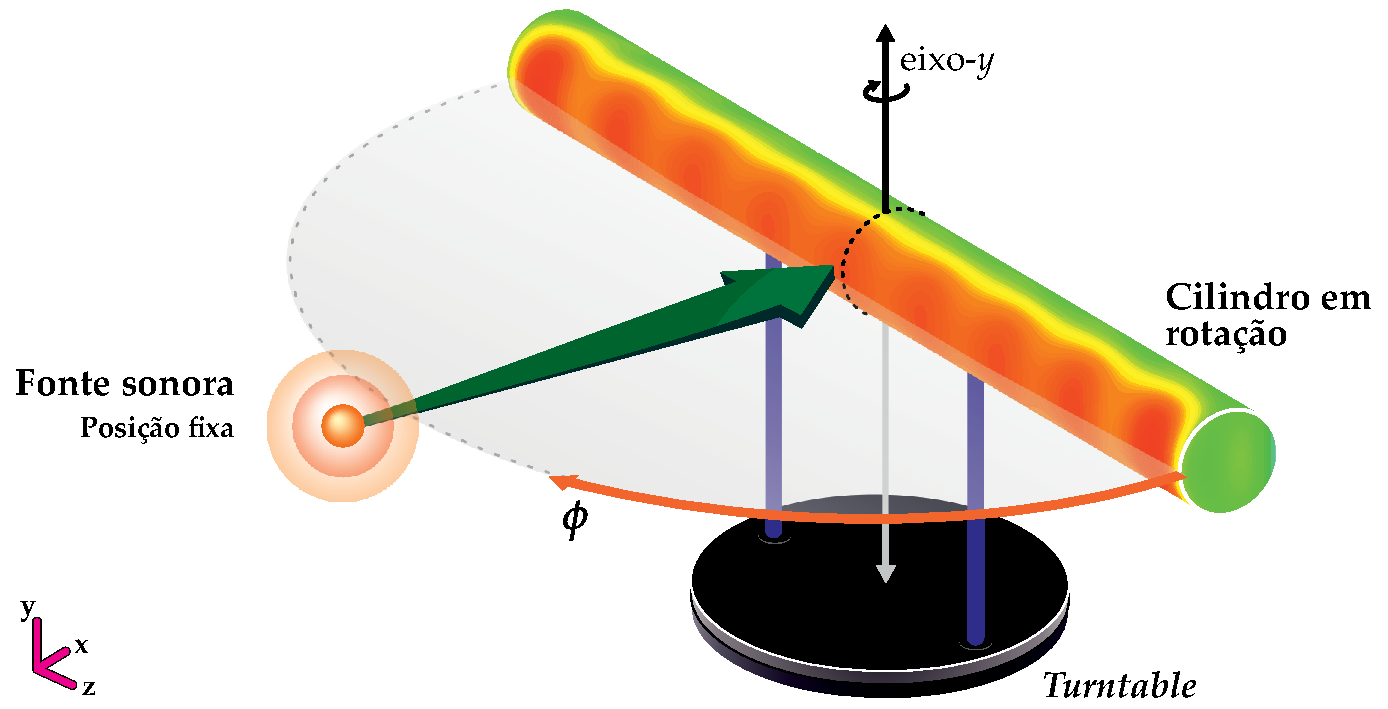
\includegraphics[width=0.74\linewidth]{figs/Measurement-Scheme-Fonseca-2013.pdf}%
	\caption{Medição de \textit{beamforming} com arranjo cilíndrico (adaptado de Fonseca \cite{Fonseca-2013}).\\ Exemplo de figura em duas colunas.}%
	\label{fig:beamforming}%
\end{figure*}

Serão adotadas as unidades do Sistema Internacional (SI). Ao escrever seu trabalho em português ou espanhol, nos números, \textbf{use o separador decimal vírgula} (conforme a língua portuguesa e espanhola vigente) seja no texto, tabelas, figuras e/ou gráficos, além de buscar sempre o uso de uma mesma precisão ao comparar números, por exemplo: 3,0 é diferente de 3,00, porém tem a mesma precisão de 6,0. 
No caso do trabalho ser escrito em inglês, fica a critério do autor usar ponto ou vírgula como separador decimal (desde que não misture as notações).
Ao escrever um número com sua unidade\footnote{Unidades são sempre grafadas ``em pé'', ou seja, não em itálico, por exemplo, 30~N/m$^2$.}, mantenha sempre o número junto à correspondente unidade, sem que exista quebra de linha entre eles (no Ms Word utilize Ctrl + Shift + Espaço, no \LaTeX\xspace coloque um til ($\sim$) entre o número e a unidade). Por exemplo, 3~m de distância separa a entrada e a saída; 4.512,28~cm é a distância medida.

As equações deverão estar encaixadas entre o texto (no Word use uma ``tabela'' simples) conforme o exemplo da Equação~\eqref{eq:area-circ}. Deverão ainda estar centralizadas e numeradas sequencialmente, com a numeração colocada no lado direito e entre parênteses (vide exemplo). Lembre-se que elas são elementos textuais, logo devem ser pontuadas e o texto conseguinte normalmente não se inicia com letra maiúscula. Recomenda-se colocar a nomenclatura imediatamente após a variável apresentada.

A área do círculo (em m$^2$) é dada por 
\begin{equation}
	A = \pi \, r^2\;,
\label{eq:area-circ}
\end{equation}
%
em que $r$ é o raio em metros (m). Lembre-se que variáveis (como o $r$ nesse exemplo) são grafadas em \textit{itálico} (seja na equação ou no texto). Porém, \textbf{unidades, funções e operadores matemáticos são escritos ``em pé''}, sem a aplicação do itálico. Por exemplo, 32,0~N/m$^2$ foi a pressão aplicada, ou ainda
%
\begin{equation}
	\int_a^b p(\phi)\, \dt p\,
\label{eq:int}
\end{equation}
%
foi a integral calculada (observe que o operador diferencial ``$\tx{d}$'' está em pé), para cada ângulo $\phi$ em graus. Como funções, pode-se citar o seno, $\sen(\theta)$, ou ainda $\log(y)$, por exemplo. 
%

Texto subscrito e sobrescrito somente será em itálico se for correspondente a alguma variável pertinente. Caso seja um ``nome complementar'', a variável deve ser colocada em pé, por exemplo, $P\txu{total}$ corresponde à pressão total em Pa, ou ainda $S\txup{\,tri}$ corresponde à área do triângulo em cm$^2$. Porém, em se tratando de uma variável, por exemplo, $i$ deve-se escrever: o somatório foi calculado considerando $P_i$ até a $i$-ésima pressão final correspondente a 256.

Caso texto, siglas ou unidades sejam utilizados em equações, sua representação deve ser em pé, por exemplo:
%
\begin{equation}
	\text{densidade} = \frac{\tx{massa}}{\;\;\tx{volume}\;\;}\,,
\label{eq:densidade}
\end{equation}

sendo que no SI (Sistema Internacional de Unidades) a unidade de densidade é o quilograma por metro cúbico (kg/m$^3$).
%

No texto, quando for necessário citar uma equação já apresentada, deve-se fazê-lo da seguinte forma: Equação~\eqref{eq:densidade} --- com apenas a primeira letra em maiúsculo e com o número correspondente entre parênteses.

%%%%%%%%%%%%%%%%%%%%%%%%%%%%%%%%%%%%%%%%%%%%%%%%%%%%%%%%%%%%%%%%%%%%%%%%%%%%%%%%%%%%%%%%%%%%%%%%%%%%%%%%%%%%%%%%%%%
\subsection{Figuras, tabelas, quadros e códigos}



As figuras e tabelas devem ser inseridas durante o texto, preferencialmente em seguida aos parágrafos a que se referem. Uma menção
às figuras, tabelas, quadros e códigos no texto corrido, antes da sua apresentação, é necessária para a orientação do leitor. As figuras, tabelas e quadros devem conter todos os elementos de formatação e de conteúdo para que sejam interpretados corretamente, sem necessidade de se recorrer ao texto corrido para uma busca de informações adicionais. Deve-se separar do texto as tabelas e figuras com \textbf{1 linha} em branco antes e depois (12~pt). 

% No Latex isso já está configurado automaticamente.

\begin{table*}[!b]
  \centering \ratb{1.3} 
  \caption{Propriedades microgeométricas e macroscópicas das camadas porosas CPA 1 e CAUQ-B \cite{Mareze-2017}.\\ Exemplo de tabela em duas colunas.}
	\fontsize{11}{12}\selectfont 
    \begin{tabular}{C{2.8cm} | C{1.5cm} | C{1.5cm} | C{1.5cm} | C{1.5cm} | C{1.5cm} | C{1.0cm}| C{1.0cm}}
    \toprule
		\SetRowColor{LightOrange}
    \textbf{ Amostra / Parâmetro } & $L\txu{p}$ \qquad [$\upmu$\! m] & $L\txu{a}$ \qquad [$\upmu$\! m] & $D\txu{p}$ \qquad [$\upmu$\! m] & $D\txu{a}$ \qquad [$\upmu$\! m] & $\sigma$ [Ns/m\txup{4}] & {$\phi$\quad [--]} & $\alpha_{\infty}$ [--]\\
	  \midrule
		CPA 1 -  3\% &	1359,81 & 1492,51 & 2344,05 & 1425,67 &	5131 &	0,218 &	1,63\\
		\rowcolor[gray]{.95} CAUQ-B - 4,5\%	& 1598,29 &	701,24 & 2126,46 & 895,34 &	54989 &	0,070 &	2,89\\
    \bottomrule
    \end{tabular}
    \label{tab.exemplo}%
\end{table*}%

As figuras, tabelas e quadros deverão ser centralizados e numerados sequencialmente (vide exemplo nas Figuras~\ref{fig:beamforming}, \ref{subfig.exemplo} e \ref{fig:C80}; Tabela~\ref{tab.exemplo}; Quadro~\ref{quad.exemplo} e Código~\ref{code.matlalatex}). Elas poderão ser colocadas em uma ou duas colunas dependendo de seu conteúdo. No caso de duas colunas, recomenda-se o posicionamento no topo ou na parte inferior da página. Busque utilizar figuras e gráficos em que seu conteúdo possa ser completamente compreendido. 

O rótulo e número das figuras, seguido da legenda, deve aparecer logo abaixo e centralizado (10~pt). Caso utilize figuras de outros autores (ou fontes), mesmo que adaptadas, indique a fonte logo após a legenda descritiva, vide exemplo da Figura~\ref{fig:beamforming}.

O rótulo, número e legenda das tabelas (quadros e códigos também) devem aparecer centralizados na parte superior (vide Tabela~\ref{tab.exemplo}). A fonte (quando necessário) das tabelas deve ser apresentada de acordo com a publicação original. A Tabela~\ref{tab.exemplo} apresenta um exemplo do estilo a ser utilizado (o conteúdo da tabela poderá conter tipografia menor que a do texto). Ademais, recomenda-se fortemente o sistema de referências cruzadas automatizado. Lembre-se que todos os objetos, como figuras e tabelas, devem ser citados no texto.

\begin{figure}[H]
  %\ContinuedFloat %% para continuar a partir da figura anterior
  \centering
	\subfloat[Figura A]{\label{fig.figA}
\includegraphics[height=23mm,page=2]{FIA-logo.pdf}}
	\qquad
  \subfloat[Figura B]{\label{fig.figB}
\includegraphics[height=23mm,page=2]{FIA-logo.pdf}}	
  \caption{Exemplo de figuras lado a lado.}
  \label{subfig.exemplo}
\end{figure}

\begin{figure}[ht!]
	\centering \vspace{-3mm}
        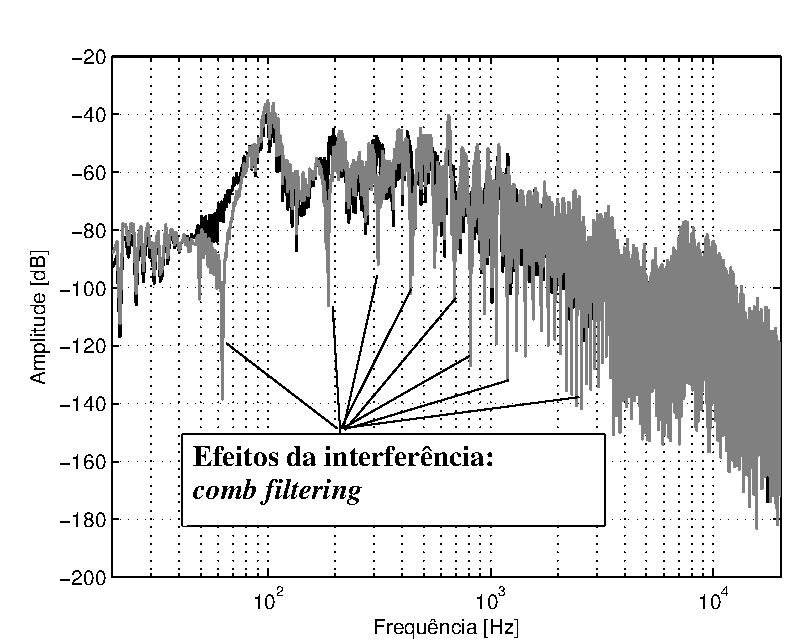
\includegraphics[width=0.98\linewidth,page=1]{figs/Combfilter-Brandao-2017.pdf}
        \caption{$C_{80}$ para salas distintas. As figuras podem ser colocadas lado a lado (retirado de Brandão \cite{Brandao-2017}).}
	\label{fig:C80}%
\end{figure}


\begin{quadro}[ht!]
%\vspace{-2mm}
  \centering \ratb{1.3} \setlength\aboverulesep{0pt} \setlength\belowrulesep{0pt}
  \caption{Este é um exemplo de um quadro.}
	\fontsize{11}{12}\selectfont 
    \begin{tabular}{| C{2.8cm} | C{1.8cm} | C{1.8cm} |}
    \hline
	\SetRowColor{LightBlue}
    \textbf{ Experimento / Tipo } & \textbf{Exp. 1} & \textbf{Exp. 2}\\
	\midrule
		Tipo 1& Verde & Amarela\\
		\rowcolor[gray]{.95} Tipo 2 & Azul & Branco\\
    %\bottomrule
		\hline
    \end{tabular}
    \label{quad.exemplo}%
% 	\vspace{-4mm}
\end{quadro}%


%% Modelo de figuras lado a lado usando minipage
%\begin{figure*}[b]
    %\centering
    %\begin{minipage}[t]{.48\textwidth}
        %\centering
        %
\includegraphics[width=1\linewidth,page=2]{FIA-logo.pdf}
        %\caption{Figura do lado esquerdo.}
        %\label{fig:ladoE}
    %\end{minipage}%
		%\quad
    %\begin{minipage}[t]{0.48\textwidth}
        %\centering
        %
\includegraphics[width=1\linewidth,page=2]{FIA-logo.pdf}
        %\caption{Figura do lado direito.}
        %\label{fig:ladoD}
    %\end{minipage}
%\end{figure*}

Recomenda-se que gráficos, figuras, fotos e qualquer arquivo gráfico, estejam inseridos no texto em formato .jpg e/ou .png com boa qualidade (ou ainda em formato vetorial em .pdf para usuários do \LaTeX\xspace). Atente para que os elementos de gráficos e figuras sejam legíveis (sobretudo se a informação for pertinente).

A distribuição deste \textit{template} de \LaTeX\xspace inclui o pacote \ttc{Codes2Latex.sty}\footnote{O pacote está ainda desenvolvimento (sem documentação detalhada), logo, para mais detalhes consulte o arquivo \ttc{sty}.}, que habilita possibilidades para documentação de códigos genéricos e nas linguagens Matlab, Fortran, Python, LabView e Latex de forma organizada (observe o Código~\ref{code.matlalatex}).

\begin{matlabcode}[Fazendo o Matlab escrever Latex.]{code.matlalatex}
  syms x
  f = taylor(log(1+x));
  latex(f)
\end{matlabcode}

Todos os elementos (figuras e gráficos, por exemplo) podem ser coloridos ou em tons de cinza. Evite a utilização de elementos textuais de outros autores sem a devida citação (e/ou autorização). É essencial que as figuras que apresentarem texto estejam na mesma língua do artigo. Não serão aceitas citações indiretas como \textit{Google imagens}, por exemplo, assim como recomenda-se evitar o uso de bases de conhecimento voláteis.

As referências cruzadas devem ser feitas para todos os elementos, por exemplo: Figura~\ref{fig:beamforming} e Tabela~\ref{tab.exemplo} (apenas a primeira letra maiúscula). Caso exista uma subfigura, use Figura~\subref*{fig.figA}, por exemplo.


%%%%%%%%%%%%%%%%%%%%%%%%%%%%%%%%%%%%%%%%%%%%%%%%%%%%%%%%%%%%%%%%%%%%%%%%%%%%%%%%%%%%%%%%%%%%%%%%%%%%%%%%%%%%%%%%%%%
\section{Tipos de artigo}

O evento aceitará \textbf{submissões originais} (isto é, ainda não publicadas) de pesquisas científicas e aplicações de engenharia, arquitetura, áudio, física, matemática, fonoaudiologia e áreas e subáreas afins. Assim, serão considerados os seguintes tipos de documento:
%
\begin{itemize}[noitemsep,topsep=-1ex] \itemsep=7pt
	\item \textbf{Artigos técnicos e aplicados} (\textit{Technical and applied papers}):
	apresentam material original a partir de aplicações de técnicas conhecidas e/ou em desenvolvimento. Deve apesentar métodos aplicados que estejam de acordo com normativas e/ou que apresentem resultados pertinentes. É essencial que sejam de interesse de pesquisadores e profissionais do tema proposto.
	
	\item \textbf{Artigos científicos} (\textit{Scientific papers}): 
	contém material original (ideias, modelos, experimentos \etc) não publicado, que contribui substancialmente para o avanço da ciência naquele tema. Ele deve estabelecer uma relação entre seu conteúdo e o \textit{estado da arte} já publicado. 
	

	\item \textbf{Artigos de revisão} (\textit{Review papers}):
	discutem o \textit{estado da arte} sobre o tema pretendido, aclarando desde aspectos básicos até os sofisticados. Esse tipo de submissão deve ser completo no que concerne à literatura, cobrindo em boa parte as ideias, modelos, experimentos \etc já desenvolvidos, mesmo que não estejam de acordo com a opinião do autor. É importante que o assunto seja de interesse da comunidade científica.	
\end{itemize}

\vspace{5pt}

As áreas temáticas do evento incluem:
%	
\begin{itemize}[noitemsep,topsep=-1ex] \itemsep=1.5pt
\item[\textbullet] Acústica geral; 
\item[\textbullet]Acústica Ambiental
\item[\textbullet]Acústica da Audição e da Fala;
\item[\textbullet]Acústica de Salas;
\item[\textbullet]Acústica de Edificações;
\item[\textbullet]Acústica Musical;
\item[\textbullet]Acústica Submarina;
\item[\textbullet]Acústica Veicular;
\item[\textbullet]Acústica Virtual;
\item[\textbullet]Aeroacústica;
\item[\textbullet]Áudio e Eletroacústica;
\item[\textbullet]Bioacústica;
\item[\textbullet]Controle de Ruído;
\item[\textbullet]Ensino em Acústica;
\item[\textbullet]Medições em acústica e vibrações;
\item[\textbullet]Legislação e normalização em Acústica;
\item[\textbullet]Materiais acústicos;
\item[\textbullet]Métodos Numéricos em Acústica e Vibrações;
\item[\textbullet]Paisagens sonoras;
\item[\textbullet]Processamento de Sinais;
\item[\textbullet]Psicoacústica;
\item[\textbullet]Ruído e vibrações em ambiente laboral;
\item[\textbullet]Ultrassom; 
\item[\textbullet]Vibrações e Vibroacústica; e
\item[\textbullet]INAD e IYS2020.
	\end{itemize}
	

%%%%%%%%%%%%%%%%%%%%%%%%%%%%%%%%%%%%%%%%%%%%%%%%%%%%%%%%%%%%%%%%%%%%%%%%%%%%%%%%%%%%%%%%%%%%%%%%%%%%%%%%%%%%%%%%%%%
%%%%%%%%%%%%%%%%%%%%%%%%%%%%%%%%%%%%%%%%%%%%%%%%%%%%%%%%%%%%%%%%%%%%%%%%%%%%%%%%%%%%%%%%%%%%%%%%%%%%%%%%%%%%%%%%%%%
\section{Organização do trabalho}

A estrutura do artigo deverá contemplar pelo menos os seguintes itens:
%
\begin{itemize}[noitemsep,topsep=0ex] \itemsep=3pt
	\item Introdução: visão geral sobre o assunto com definição dos objetivos do trabalho, indicando a sua relevância.
	\item Fundamentos: sobretudo em artigos científicos, a fundamentação teórica principal necessária ao entendimento do texto deve ser apresentada e referenciada; 
	\item Desenvolvimento: como o trabalho foi realizado, incluindo detalhes de teoria, materiais e métodos empregados;
	\item Resultados e discussões: parciais ou conclusivos, conforme a modalidade do trabalho, fazendo referência a medições e cálculos estatísticos aplicados, se for o caso;
	\item Conclusões ou Considerações finais: basear-se nas discussões e objetivos, apresentando apontamentos e considerações que findam o estudo/aplicação;
	\item Agradecimentos: opcional, quando for pertinente;
	\item Referências: apresentar bibliografia citada no texto.
\end{itemize}
%
Não é preciso necessariamente existir seções com estes nomes. A organização é também dependente do tipo do artigo.
Outros elementos pós-textuais como apêndices são opcionais, desde que eles (no total) não excedam o limite total de 12 páginas. 

%%%%%%%%%%%%%%%%%%%%%%%%%%%%%%%%%%%%%%%%%%%%%%%%%%%%%%%%%%%%%%%%%%%%%%%%%%%%%%%%%%%%%%%%%%%%%%%%%%%%%%%%%%%%%%%%%%%
\subsection{Citações e referências}

Para a confecção das referências deve-se utilizar a norma vigente. As referências devem ser \textbf{numeradas conforme ordem de aparição}, utilizando colchetes \cite{Gomes-2015}. Todas referências devem ser citadas durante o texto. As referências \cite{Mareze-2017,Fonseca-2013,Brandao-2017,Gomes-2015,Oppenheim-2010,Muller-2001,Mareze-2019,Borges-2018,Ristow-2016} deste modelo de artigo são apenas ilustrativas (para efeito de compreensão).

% No Latex, recomenda-se usar unsrtnat e unsrtnat-br.

Ao final do documento a seção de referências deve ser colocada. As entradas nela contidas devem ter tipografia com tamanho 10~pt, espaçamento simples e espaçamento de parágrafo de 6~pt. Este \textit{template} de \LaTeX\xspace usa o pacote {\ttfamily natbib} para a organização das referências. Além disso, recomenda-se a utilização de gerenciadores de banco de dados de bibliografia como o \href{http://www.jabref.org/}{JabRef}, \href{http://www.mendeley.com}{Mendeley} e \href{https://www.zotero.org/}{Zotero}. Em especial para usuários do Word, o Mendeley tem um \textit{plugin} para formatar e inserir as referências no documento .docx.



Dependendo do contexto, o nome do autor pode ou não ser escrito, conforme os exemplos a seguir: 
%
\begin{itemize}[noitemsep,topsep=0ex] \itemsep=4pt
	\item 	``... Mareze et al. \cite{Mareze-2019} trabalharam com absorção de materiais porosos...'' ou 
	
	\item ``... para o estudo de acústica de salas \cite{Brandao-2017} recomenda-se a leitura de um livro texto...'' ou
	\item ``... aplicando a Transformada de Fourier nos sinais de entrada \cite{Oppenheim-2010}. '' ou ainda
	\item ``... Fonseca (2013) demonstrou o cálculo de difração para superfícies cilíndricas~\cite{Fonseca-2013}.''
\end{itemize}
%
Todos os autores que constam nas referências devem estar citados no texto.

Em referências com até três autores, por exemplo, Müller e Massarani \cite{Muller-2001}, ambos devem ser citados (quando evocados). No caso de mais de três autores, por exemplo, Gomes \etal \cite{Gomes-2015} deve-se citar somente o último nome do primeiro autor seguido da expressão ``\etal''. Ainda, ao citar mais de uma referência, utilize apenas um colchete, veja alguns exemplos a seguir:
%
\begin{itemize}[noitemsep,topsep=0ex] \itemsep=8pt
	\item 	``Trabalhos em temas de acústica e vibrações \cite{Mareze-2017,Fonseca-2013,Brandao-2017}.''
	\item ``Trabalhos em temas de acústica \cite{Mareze-2017,Oppenheim-2010,Muller-2001,Mareze-2019}.''
	\item ``Trabalhos com análise estatística \cite{Mareze-2017, Brandao-2017, Borges-2018}.''
		\item \textbf{Não usar esse estilo:} ``Trabalhos com análise estatística \cite{Mareze-2017}, \cite{Brandao-2017}, \cite{Ristow-2016}.''
\end{itemize}
%
Recomenda-se que a referências sejam ordenadas e compactadas (com meia-risca) como em \cite{Mareze-2017,Oppenheim-2010,Muller-2001,Mareze-2019}.

Na seção de referências, sempre que possível, inclua o ISBN, ISSN, DOI\footnote{Para usuários de Latex basta usar o campo ``doi'' de seu \texttt{.bib}.} (com link) e/ou link com a direção online em que o documento citado está disponível.

%%%%%%%%%%%%%%%%%%%%%%%%%%%%%%%%%%%%%%%%%%%%%%%%%%%%%%%%%%%%%%%%%%%%%%%%%%%%%%%%%%%%%%%%%%%%%%%%%%%%%%%%%%%%%%%%%%%
\section{Submissão e avaliação}

Após a aprovação dos resumos submetidos no site do evento: \url{http://fia2020.com.br}, os autores serão convocados para elaborar os trabalhos completos.
Detalhes acerca de registro podem ser consultado também no site, ou com a comissão organizadora.

É responsabilidade dos autores a preparação e envio dos artigos em seu formato final. Por esse motivo, pede-se que verifiquem com atenção a formatação de seus artigos, especialmente gráficos e fotos, quanto à legibilidade e qualidade digital (e para impressão). \textbf{Os artigos deverão ser enviados em formato PDF (com tamanho máximo de 10~Mb).} 

Os metadados do PDF para usuários de \LaTeX\xspace são feitos automaticamente, usuários de MS Word devem conferir no momento da conversão.

% Uso de PDF-a fica opcional.

Pesquisas que envolvam pessoas (ou seres vivos, em geral), como em acústica subjetiva ou fisiológica, por exemplo, deverão aclarar no artigo o termo de aprovação do Comitê de Ética, caso pertinente.

%%%%%%%%%%%%%%%%%%%%%%%%%%%%%%%%%%%%%%%%%%%%%%%%%%%%%%%%%%%%%%%%%%%%%%%%%%%%%%%%%%%%%%%%%%%%%%%%%%%%%%%%%%%%%%%%%%%
\section{Modelos para Word e \LaTeX}

O modelo de \LaTeX\xspace (\texttt{.tex}) foi escrito em codificação UTF8, assim é compatível com Windows, Mac, Linux e \href{https://www.overleaf.com/read/rnfjxkknksnd}{Overleaf}\footnote{\url{https://www.overleaf.com/read/rnfjxkknksnd}.}. Pode ser usado livremente para a elaboração dos artigos.

O modelo de \texttt{.docx} foi criado em Microsoft Word 2016 e, com isso, suas funcionalidades de espaçamento e configurações são garantidas para essa versão.

O autor deste texto (em português) e dos modelos é o professor William D'Andrea Fonseca, da Engenharia Acústica (EAC) da Universidade Federal de Santa Maria (UFSM).\linebreak
A revisão foi realizada pelo professor {Stephan Paul} (UFSC).
O modelo de MS Word foi finalizado pelo professor Rafael Heissler (Unisinos).

% A versão em espanhol foi traduzida por \hw{Cicrano com revisão de Fulano}. 
% A versão em inglês foi traduzida por \hw{Cicrano com revisão de Fulano}.

Todas eles estão disponíveis com links no \href{http://fia2020.com.br}{site do evento}, no \href{https://www.overleaf.com/read/rnfjxkknksnd}{Overleaf} e no \href{https://github.com/willdfonseca/fia2020}{GitHub}\footnote{\url{https://github.com/willdfonseca/fia2020}.}.

%%%%%%%%%%%%%%%%%%%%%%%%%%%%%%%%%%%%%%%%%%%%%%%%%%%%%%%%%%%%%%%%%%%%%%%%%%%%%%%%%%%%%%%%%%%%%%%%%%%%%%%%%%%%%%%%%%%
\section{Considerações finais}

Busca-se, por meio desse \textit{artigo modelo}, elencar e aclarar as instruções para submissão de artigos para o FIA 2020 integrando o XXIX Encontro da Sobrac. 
Este próprio documento pode ser usado como modelo apenas trocando o conteúdo.

%%%%%%%%%%%%%%%%%%%%%%%%%%%%%%%%%%%%%%%%%%%%%%%%%%%%%%%%%%%%%%%%%%%%%%%%%%%%%%%%%%%%%%%%%%%%%%%%%%%%%%%%%%%%%%%%%%%
\section{Agradecimentos}

Se for pertinente, faça agradecimentos.
%
Em caso de trabalhos com fomento, utilize esta seção para elucidar detalhes.

No caso deste documento, gostaríamos de agradecer à cooperação de todos para com o evento.
%%%%%%%%%%%%%%%%%%%%%%%%%%%%%%%%%%%%%%%%%%%%%%%%%%%%%%%%%%%%%%%%%%%%%%%%%%%%%%%%%%%%%%%%%%%%%%%%%%%%%%%%%%%%%%%%%%%%
%%%%%%%%%%%%%%%%%%%%%%%%%%%%%%%%%%%%%%%%%%%%%%%%%%%%%%%%%%%%%%%%%%%%%%%%%%%%%%%%%%%%%%%%%%%%%%%%%%%%%%%%%%%%%%%%%%%%
%%% Referências
\renewcommand{\refname}{Referências} \addcontentsline{toc}{section}{\refname}% 
% \bibliographystyle{unsrtnat} 
\bibliographystyle{unsrtnat-br}  % Estilo semelhante ao padrão brasileiro
{{\fontrefs \bibliography{bibliografia}}
%%%%%%%%%%%%%%%%%%%%%%%%%%%%%%%%%%%%%%%%%%%%%%%%%%%%%%%%%%%%%%%%%%%%%%%%%%%%%%%%%%%%%%%%%%%%%%%%%%%%%%%%%%%%%%%%%%%
%%%%%%%%%%%%%%%%%%%%%%%%%%%%%%%%%%%%%%%%%%%%%%%%%%%%%%%%%%%%%%%%%%%%%%%%%%%%%%%%%%%%%%%%%%%%%%%%%%%%%%%%%%%%%%%%%%%
\appendix
\section{Exemplo de apêndice}

Este é um exemplo de apêndice, geralmente se colocam informações adicionais ou derivações produzidas pelos autores.

Este modelo (\textit{template} de \LaTeX) tem alguns comandos adicionais que facilitam a escrita, como, por exemplo, \F\xspace para simbolizar a Transformada de Fourier. Para conhecer melhor os comandos, consulte o arquivo \texttt{FIA2020.sty}.

%%%%%%%%%%%%%%%%%%%%%%%%%%%%%%%%%%%%%%%%%%%%%%%%%%%%%%%%%%%%%%%%%%%%%%%%%%%%%%%%%%%%%%%%%%%%%%%%%%%%%%%%%%%%%%%%%%%
%%%%%%%%%%%%%%%%%%%%%%%%%%%%%%%%%%%%%%%%%%%%%%%%%%%%%%%%%%%%%%%%%%%%%%%%%%%%%%%%%%%%%%%%%%%%%%%%%%%%%%%%%%%%%%%%%%%
% Exemplo de códigos em duas colunas
%\onecolumn
%\section{Escrevendo um código de apêndice em uma coluna}
%
%Caso existam códigos muito extensos, o apêndice pode ser convertido para uma coluna, como exemplificado nesta seção com o Código~\ref{code.fc}.
%
%\inputcodeLatin{Matlab}{Exemplo de inclusão de código (de Matlab) em duas colunas.}{code.fc}{FC.m}

%%%%%%%%%%%%%%%%%%%%%%%%%%%%%%%%%%%%%%%%%%%%%%%%%%%%%%%%%%%%%%%%%%%%%%%%%%%%%%%%%%%%%%%%%%%%%%%%%%%%%%%%%%%%%%%%%%%
% \clearpage  \listoftodos % This temporary list may help the writing of the paper.
%%%%%%%%%%%%%%%%%%%%%%%%%%%%%%%%%%%%%%%%%%%%%%%%%%%%%%%%%%%%%%%%%%%%%%%%%%%%%%%%%%%%%%%%%%%%%%%%%%%%%%%%%%%%%%%%%%%
%%%%%%%%%%%%%%%%%%%%%%%%%%%%%%%%%%%%%%%%%%%%%%%%%%%%%%%%%%%%%%%%%%%%%%%%%%%%%%%%%%%%%%%%%%%%%%%%%%%%%%%%%%%%%%%%%%%
\end{document}
%%%%%%%%%%%%%%%%%%%%%%%%%%%%%%%%%%%%%%%%%%%%%%%%%%%%%%%%%%%%%%%%%%%%%%%%%%%%%%%%%%%%%%%%%%%%%%%%%%%%%%%%%%%%%%%%%%%
% EOF